
\chapter{Brief summary of the state of the art of ultrasound probing for liquid sodium}

In this chapter, let us introduce the general context of the thesis, and its main goals.
In \autoref{ssec:gen4} we will thus briefly recall some international research and development projects related to the new fourth-generation nuclear
reactors, which is the background of this thesis. Then in \autoref{ssec:ac_nuc} we will recall how ultrasound measurement techniques are
used in nuclear reactors. We will indicate methods that have been proposed in past research projects. In the following sections (\autoref{ssec:ac_char}), the acoustic
properties of the coolant medium (i.e. liquid sodium) of the SFRs are presented. The heterogeneous thermo-fluidal state of the medium in an operating
situation of the reactor is explained, referring to former studies, in \autoref{sec:stat_sod}. Finally the possible effects of heterogeneity of the medium
on acoustic wave propagation, which are discussed in the literature, and the objectives of this thesis will be explained (\autoref{ssec:fluc_mod} and \autoref{sec:goals}).

\section{Sodium-cooled fast reactors and the need for ultrasound measurements}

\subsection{The Generation-IV forum and ASTRID project} \label{ssec:gen4}

    Research \& development (R\&D) of next-generation nuclear power systems is being pursued under the "Framework agreement for international collaboration on
research and development of generation IV nuclear energy systems" by countries belonging to the Generation IV International Forum (GIF)
\citet{GIF2005Frameworkagreementfor}. Initially, in 1999, the United States advocated the concept of Generation-IV nuclear reactors and then proposed to other
countries to organize an international forum for international collaboration to develop fourth-generation nuclear power systems. In response to this, in July
2001, a charter that defines the principles of GIF was formalized by the Republic of Argentina, Brazil, Canada, France, Japan, the Republic of Korea, South
Africa, the United Kingdom and the United States. After subscriptions by the European Atomic Community (i.e. Euratom), People's Republic of China, Russia and
Switzerland, GIF is nowadays being operated by 12 countries and one international organization.

    Generation IV (Gen-IV) is defined as a new nuclear power system following the nuclear reactors at the beginning of nuclear reactor technology from the 1950's
to the first half of the 1960's (Gen-I), commercial light-water reactors built from the latter half of the 1960's to the first half of the 1990's (Gen-II) and their improved
versions from the latter half of the 1990's to the 2010's (Gen-III and Gen-III+). The objectives of GIF were clearly identified as:
    \begin{itemize}
     \item achieve sustainable development of nuclear energy by optimizing the use of natural uranium resources and by reaching the highest levels of nuclear safety,
     \item minimize the production of the most radioactive waste, in particular long-lived waste,
     \item ensure high resistance to nuclear proliferation,
     \item develop applications of nuclear energy for other uses than production of electricity.
    \end{itemize}
    After the analysis phase for designing plans, the GIF consortium selected six concepts of nuclear reactors that exhibited promising potentials to
achieve the above-mentioned objectives \parencite{GIF2014TechnologyRoadmapUpdate}.
    \begin{itemize}
     \item SFR: Sodium-cooled Fast Reactor
     \item GFR: Gas-cooled Fast Reactor
     \item LFR: Lead-cooled Fast Reactor
     \item SCWR: Supercritical Water-cooled Reactor
     \item VHTR: Very High Temperature Reactor
     \item MSR: Molten Salt Reactor.
    \end{itemize}
    Advantageous thermo-physical properties of the coolant, liquid sodium for SFR concept leading to normal atmospheric pressure, (i.e. high boiling point, heat of vaporization, heat capacity and thermal
conductivity) lead to a large safety margin for coolant boiling, and this contributes to important safety features of Sodium-Cooled Fast Reactors (SFRs), which
is one of the design purposes of Gen-IV nuclear reactors. Thus, SFR was adopted as one of the possibilities for Gen-IV, and its R\&D is carried out
internationally in France, Japan, Russia, USA, Republic of Korea and China. This limited number of countries implied in SFR explains the small number of international references
in the bibliography.

    Before GIF, the development of SFR has been undertaken in many countries through operations of several experimental, prototype and demonstration reactors,
for example Rapsodie, Phenix, SuperPhenix in France, PFR in the United Kingdom, BN-550, BN-600 and BN-800 in Russia and Monju and Joyo in Japan.
    In France, an R\&D project aimed at technological innovation concerning SFR has now been launched in collaboration with the French Alternative Energies and
Atomic Energy Commission (CEA), Areva (now called Framatome) and Electricity de France (EDF) in 2007. As a part of this global project, a first prototype industrial-sized SFR
development is ongoing. It is called the ASTRID project (Advanced Sodium Technological Reactor for Industrial Demonstration). This project pursuits four technical
targets \parencite{CEA20124thgenerationsodium}:

    \begin{figure}[htbp]
        \centerline{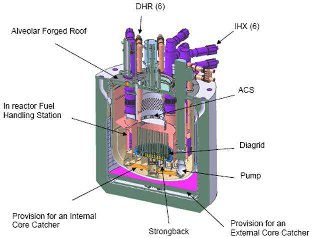
\includegraphics[width=10.0cm]{design_astrid.pdf}}
        \slantedcaption{
        Pre-conceptual design for the ASTRID reactor block (taken from \cite{Baque2015ASTRIDInService}).
        DHR: Decay Heat Removal system.
        IHX: Intermediate Heat Exchanger, which transfers heat from the primary coolant circuit to the secondary coolant circuit.
        ACS: Above-Core Structure, which supports the control rod drive mechanisms and core instrumentation, including the thermocouples etc.
        Internal/external core catcher: Collect and manage the corium (melted core and metallic structure) in case of a Core Disruptive Accident.
        Strongback: Structure in sodium coolant that supports the core.
        Diagrid: Structure that supports the subassemblies.}
        \label{fig:design_astrid}
    \end{figure}

    \begin{itemize}
       \item  Design of a high-performance core with improved safety: in particular, concerning prevention of severe accidents likely to cause complete core
meltdown,
       \item  Improved resistance to severe accidents and external aggressions: in particular, design of redundant and diversified decay heat removal systems,
as well as aspects related to the risk of re-criticality accident (i.e. uncontrolled nuclear fission chain reaction) and to molten core containment,
       \item  Search for an optimized and safe power conversion system intended to reduce or even completely remove the risk of interaction between sodium and
water,
       \item  Reactor design options to make inspection and maintenance easier and, more generally, to improve the availability, performance and general
economic characteristics of the facility
       (Figure \ref{fig:design_astrid} shows the pre-conceptual design of the planned ASTRID reactor).
    \end{itemize}
    Because of their high reactivity with sodium, the coolant circuit of SFR needs to be completely sealed from air and water, thus
further development of inspection and monitoring techniques are one of the keys for practical applications of SFR \parencite{GIF2014TechnologyRoadmapUpdate}.

\subsection{Ultrasound as a monitoring technique for ASTRID for in-service inspection and repair and for continuous surveillance} \label{ssec:ac_nuc}

    We give below a short summary of acoustic applications that are being developed in the framework of the ASTRID project (see e.g. \parencite{Giot2017Nuclearinstrumentationmeasurement}).
Similar developments have been or are being made in other frameworks; some of them will be reported in this dissertation.
    Schematically, two main reactor environmental conditions are to be considered:
    \begin{itemize}
    \item Operation periods, which are associated with high temperature (550\textdegree{}C approx.), high coolant flow, and high levels or radiation (neutron plus gamma),
    \item Shutdown periods, which are associated with lower temperature (200\textdegree{}C approx.), lower coolant flow, and lower levels of radiation.
    \end{itemize}
    In the field of applications, two domains are also classically considered:
    \begin{itemize}
    \item In-Service Inspection and Repair (ISI\&R), which is generally associated with the shutdown periods. Some typical applications are:
        \begin{itemize}
        \item non-destructive-evaluation, periodic inspection of welds,
        \item periodic inspection of structure integrity, locations and displacements of structures,
        \item imaging of objects and structures,
        \end{itemize}
    \item Continuous Surveillance (CS), which is generally associated with the operating periods.
    Some typical applications are:
        \begin{itemize}
        \item boiling detection in the primary circuit, and leakage detection in the secondary circuit,
        \item gas monitoring: sizing argon bubbles, and void fraction measurements,
        \item structure displacements,
        \item sub-assembly displacement monitoring,
        \item sub-assembly outlet temperature monitoring, ...
        \end{itemize}
    A third domain focuses on the refueling periods of the reactor, at shutdown conditions.
    Some typical applications are:
       \begin{itemize}
       \item monitoring of refueling operations versus mechanical conditions,
       \item monitoring of refueling safety versus subassembly characteristics and history, sub-assembly identification.
       \end{itemize}
    \end{itemize}

    The use of a sodium environment results in strong limitations in terms of available investigation techniques,
for the continuous surveillance / operation period conditions, as well as for the routine in-service inspection / shutdown period conditions (sodium draining is considered as an exceptional procedure, for the sake of repair for example).
    Sodium is a metallic element, with a high electrical conductivity and a magnetic behavior, and is rather opaque to electromagnetic waves.
    Magnetic and electrical fields can be induced at very short distances, for instance with Electromagnetic Acoustic Transducers (EMAT), to produce acoustic waves.
However, electromagnetic (including optical) and electrical techniques are unusable in sodium for long distance measurements, as mentioned above.

    Acoustic techniques have been regarded as convenient ones for the above purposes, in a passive "receiver" mode (noise detection of boiling and of leaks, generally at low frequencies), as well as in an active "transmitter-receiver" mode (telemetry-based measurements, generally at high frequencies).
Indeed, pure liquid sodium has rather good acoustic properties, with low attenuation and a moderate acoustic wave speed (about \SI{2400}{\meter\per\second}, with suitable wavelengths),
and acoustic techniques can thus be used in a broad frequency domain (currently up to 5 MHz for instance).
    Specific acoustic transducers have been and are still being developed to fulfill the shutdown and the operation physical conditions, as well as the acoustic specifications.

    It is known that temperature and flow heterogeneities and fluctuations will affect acoustic propagation (signal amplitude and signal-to-noise ratio, time of flight, path deflection, ...), with effects that increase with the propagation distance. These effects are far stronger in operation conditions than in shutdown conditions (which may be considered as isothermal and steady, in first stages of acoustic studies at least).

Our studies thus mostly focus on continuous surveillance conditions, and two representative applications, in the active mode, will be considered in \autoref{ssec:ac_prop} and in this dissertation:
    \begin{itemize}
    \item Ultrasonic temperature measurement at the outlet of fuel sub-assemblies (with possibly long propagation distances), which was the starting point for the studies of ultrasound propagation in heterogeneous sodium at CEA, and is studied in the general framework of SFR as a possible alternative to thermocouple-based measurements,
    \item Ultrasonic sub-assembly displacement monitoring (with shorter propagation distances), which has already been implemented in the Phenix reactor (using the SONAR device), and is studied in the framework of the ASTRID project as well.
    \end{itemize}
The description of this medium, from an acoustic point of view, is presented in the next section.

\section{Ultrasonic waves in liquid sodium}

\subsection{Properties of liquid sodium for ultrasound} \label{ssec:ac_char}

    To describe acoustic wave propagation in liquid sodium, it is necessary to know two main properties: density and wave speed. Both of them are temperature dependent.
    The characteristics of liquid sodium and its temperature-dependent properties were reported in \cite{Sobolev2011Databaseofthermophysical}. That study shows
that at normal atmospheric pressure, the density difference of liquid sodium with temperature change between the temperature range from the normal melting
point to the normal boiling point may be calculated with the linear relation:
    \begin{align}\label{eq:I_1}
        \rho\,[ \text{kg} \, \text{m}^{-3} ]=1014-0.235\cdot T\,[ \text{kelvin} ].
    \end{align}
    The sound speed of liquid sodium decreases monotonically with temperature, which is caused by decreasing of the inter-atomic interactions. In the range
of the normal melting - boiling point (\num{371}-\num{1155}\textdegree{}\si{\kelvin}), sound speed in pure liquid sodium may be described based on a linear relation:
    \begin{align}\label{eq:I_2}
        c_p\, [\text{m}\, \text{s}^{-1}] = 2723-0.531\cdot T\,[\text{kelvin}].
    \end{align}
    In this study, these two formulations are applied for acoustic properties of liquid sodium because the valid temperature range for these equations matches
the in-operation situation of the ASTRID.

    Because of these characteristics, an acoustic field may be influenced and modified by the heterogeneity of temperature in liquid sodium.
    A visualization of such modified acoustic rays can be found in the introduction part of published studies that are mentioned in the later part of this chapter (Figure \ref{fig:nicolas} in \autoref{ssec:fluc_mod} for instance).
    Variations of the acoustic impedance $Z$ ($Z=\rho c_p$) affect the transmission of ultrasonic waves (attenuation), and variations of the acoustic speed accelerate, decelerate or deviate the acoustic wave (refraction of the acoustic wave). This may lead to well-known undesirable effects when the amount of modification becomes large: degradation of the signal-to-noise ratio, focusing or defocusing of the acoustic beam, and creation of acoustic shadow zones.
What makes this matter very complex is the fact that the behavior of the heterogeneity changes spatially and temporally at the same time. Thus it is important to obtain information on the temperature state of a coolant flow when one designs acoustic devices for SFR.

%%% TODO add deflacted wave or path image

\subsection{Ultrasonic measurements in liquid sodium} \label{ssec:ac_prop}

    Several applications of acoustic measurement in liquid sodium have been studied in the literature.
    Thermometry (i.e. an acoustic telemetry technique for the measurement of temperature) is one of them. Monitoring the thermo-fluidal state of the coolant is
a very important perspective to reach a safe operation of nuclear reactors. Hence, for previous French reactors such as Phenix and Superphenix, measurement of
the sodium temperature at the core outlet was already performed based on thermocouples.

    Acoustic thermometry is not the only way to measure temperature of the upper core region i.e. the method using thermocouples, but acoustic thermometry may
be applied to SFR because of its advantages \parencite{Massacret2014Etudedunemethode}. One of the main advantages of this method is its ability to perform
high-frequency measurement; for acoustic measurements, there is no duration for heat transfer to the sensor through thermally-inert materials, which inevitably
occurs in the case of thermocouples. This ensures a very fast measurement, whose frequency may possibly be up to a few kiloHertz, which makes it possible to
monitor the fast temperature evolutions that may result from incidents or accidents. Another advantage of this method is that multiple locations on an acoustic
path may be measurable at the same time. This may reduce the number of measurement devices.

    Thermometry needs to use two reflections of an acoustic echo from reflecting objects that are present on the acoustic path. When distances between an
acoustic source and those objects are known, the average sound speed between the two objects may be calculated by
    \begin{align}\label{eq:I_3}
        c'_{ij}=\frac{2(d_i-d_j)}{t_i-t_j},
    \end{align}
    where $c'_{ij}$ is the average sound speed between the $i$-th and $j$-th reflective objects, $d_i$ is the distance from an acoustic source to the $i$-th object, and
$t_i$ is the so-called acoustic time of flight (TOF) i.e. the travel time from the emitter to the receiver. All reflection points and acoustic source are assumed to
be aligned. From equations \ref{eq:I_2} and \ref{eq:I_3}, the average temperature between two objects is estimated. Figure \ref{fig:tspatent} shows a drawing
of this concept of thermometry \parencite{McKnight1987Remotetemperaturemeasurement}.
Sub-figure A shows an application of an acoustic device (12) targeting multiple subassembly heads from above, and B shows a horizontal section view.
When the positions of the multiple subassembly heads are on a single acoustic ray, theoretically this configuration may measure the average temperature of the areas t1, t2 and t3.
C shows another example of application in which the acoustic transducer measures temperature in a single subassembly head.
If it is possible to change the angle of the transducer, a single device may measure temperature at multiple positions (D).
For 20 years, this technique was licensed as a U.S. patent no. US4655992A.
As one can see in Figure \ref{fig:tspatent}, one of the advantages of this technique is that local temperature values of multiple points
are measurable with a single acoustic device.
    \begin{figure}[htbp]
        \centerline{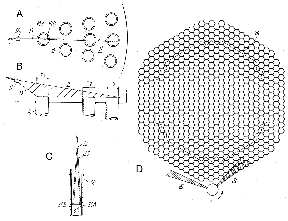
\includegraphics[width=13cm]{tspatent2.pdf}}
        \slantedcaption{Conceptual diagrams of thermometry, taken from \cite{McKnight1987Remotetemperaturemeasurement}.}
        \label{fig:tspatent}
    \end{figure}

    In 1992, ultrasonic thermometry was tested in the loop called HIPPO. HIPPO was a 1/2 scale representation of the core of a reactor of the European Fast Reactor (EFR) type
\parencite{Taylor1992Subassemblyoutlettemperature}. The objective of the experimentation was to observe the effects of a turbulent water flow on the
ultrasonic measurement of temperature at the outlet of sub-assemblies. The use of a core mock-up made it possible to determine the influence of subassembly
vibrations and potential false echoes occurring in the vicinity of assemblies. The fluid medium used in this experiment was water, and the subassembly outlets
were made of plastic. During the experiments, the flow rate in each assembly was 3.3 liter \si{\per\second}
(representing a flow speed of about \SI{1.5}{\meter\per\second}, half the real-life speed) and the water was at ambient
temperature in the whole loop. An \SI{5}{\mega\hertz} ultrasonic transducer was placed above the core and was aiming at an alignment of six
assemblies, as shown in Figure \ref{fig:hippo}. This transducer was similar to the transducers designed for actual EFRs.

    \begin{figure}[htbp]
        \centerline{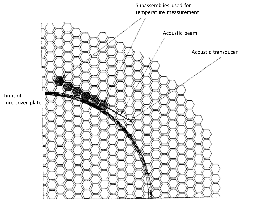
\includegraphics[width=12cm]{hippo.pdf}}
        \slantedcaption{Application of ultrasonic thermometry in the HIPPO loop, taken from \cite{Taylor1992Subassemblyoutlettemperature}.}
        \label{fig:hippo}
    \end{figure}
%
    It was verified that temperature measurement between the edges of the outlets of the sub-assemblies was possible with an uncertainty of only
$\pm$\num{0.6}\textdegree{}C, i.e. about \numrange{0.6}{2.0}\% of the average temperature (\numrange{10}{30} \textdegree{}C).
The result of this study \parencite{Taylor1992Subassemblyoutlettemperature} also indicates that
the ultrasonic measurement was not disturbed either by the flow of water nor by the potential assembly vibrations. It would have been interesting to determine
the influence of the size reduction of the geometry of the assemblies, which directly relates to the size of the thermal-hydraulic fluctuation patterns, on the
propagation of ultrasounds whose wavelength is full size (while the size of the sub-assemblies was half). Nevertheless, the accuracy of the temperature
measurements achieved by this technique, together with the absence of vibration effects, should encourage its implementation and further studies like ours.

The acoustic telemetry technique has also been used for the monitoring of the position of subassembly heads.
CEA for instance developed an acoustic measurement system called SONAR in order to study the generation mechanism of
four scrams by overpassing the reactivity threshold (an event called AURN) that occurred in the operation
of the French Phenix fast breeder reactor (FBR) \parencite{Berton1996Continuousmonitoringof}.
The objective of the SONAR system was to examine an hypothesis that AURN was caused by a small radial displacement of the subassembly.
SONAR measures the position of the subassembly head by tracking the change of time-of-flight
between the transducer surface and the subassembly head.

\begin{figure}[htbp]
    \centerline{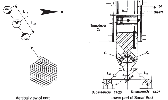
\includegraphics[width=10cm]{sonar_v2.pdf}}
    \slantedcaption{Image of the SONAR rod installation, taken from \cite{Berton1996Continuousmonitoringof}.}
    \label{fig:sonar}
\end{figure}

Figure \ref{fig:sonar} shows the description of the SONAR design.
The left image indicates the relation between the position of the SONAR rod and that of the target edges of the subassembly.
The right image is the cross-sectional image explaining the composition of the SONAR experiment.
There are multiple acoustic transducers in a rod.
C1 and C4 are used for measuring the time-of-flight to and from a subassembly edge.
The transducer C2 is used to measure the movement of the SONAR rod itself, caused by the flows.
As indicated in the left image, the acoustic ray does not pass through the central axis position of the sodium jets in this configuration,
but the effect of the medium heterogeneity occurs nonetheless for this position, as can be observed in the recorded signal in Figure~\ref{fig:sonar2}A.

\cite{Berton1996Continuousmonitoringof} show the measured signal fluctuation in the reactor at \num{550}\textdegree{}C.
The first curve in Figure \ref{fig:sonar2} is the estimated distance between the transducer and the subassembly edge for the C1 transducer.
The second curve is the measured distance between the C2 transducer and the wall of the sleeve, which indicates the movement of the SONAR rod.
The third curve is the estimated distance between C1 and the targeted subassembly edge, for which the effect of a change in the rod position is subtracted.
The noise in this curve gives an idea of the effect of thermo-hydraulic fluctuations in the SFR.
\cite{Fontaine2011Descriptionandpreliminary} studied deformation states of the subassembly and changes of fuel reactivity, and controlled the flowering (radial expansion) state
of a subassembly rod mechanically.
They measured the induced displacement of the subassembly head using the SONAR system in the Phenix reactor.
Figure \ref{fig:sonar2}B shows the radial displacement measured by the SONAR device versus their mechanical control states of subassembly flowering,
indicated as "Vertical piston position".
This is because, in the experiment device, the amount of flowering was controlled by the movement of a piston inserted in a test subassembly rod.
In this paper, the relation between the amount of flowering, the temperature of the sodium and reactivity is studied as well.
The sodium temperature was \num{350}\textdegree{}C.

\begin{figure}[htbp]
    \centerline{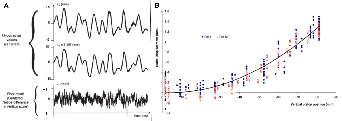
\includegraphics[width=16cm]{sonar2_v2.pdf}}
    \slantedcaption{Measured displacement of a subassembly head measured by SONAR, taken from \cite{Berton1996Continuousmonitoringof} (left) and \cite{Fontaine2011Descriptionandpreliminary} (right).}
    \label{fig:sonar2}
\end{figure}

As shown in \cite{Berton1996Continuousmonitoringof} and \cite{Fontaine2011Descriptionandpreliminary}, SONAR can thus measure small displacements of the tracked subassembly head.
The sensitivity of the measurement strongly depends on the noise created by the SONAR rod vibrations and by the thermal-hydraulic fluctuations.
Because the displacement is a short transient one, it is not possible to enhance the signal-to-noise ratio based on time-averaging techniques for example.
One must thus evaluate the error that thermal-hydraulic fluctuations can induce.
Also correcting vibratory perturbations, \cite{Berton1996Continuousmonitoringof} shows that measured distance fluctuation is
$\pm$ \SI{0.7}{\milli\meter} when the reactor is in operation (which is equivalent to a $\pm$ \num{10}\textdegree{}C temperature fluctuation).
Generally speaking, the sensitivity will depend on numerous factors:
position of the transducer, ultrasonic path (whether it passes through the hot sodium jets or not), sodium recirculation, size of the jets, and flow speed (which is itself
related to subassembly head design).
This is one of the reasons why numerical simulation can be a powerful tool to optimize devices involved in SFR studies.
One must also study the amplitude and shape of the echo, and study the elastic interaction between the subassembly head and the incident acoustic wave.
In the case of 3D circular head geometries with complex machined parts, an accurate 3D numerical simulation,
which could be performed based on the SPECFEM3D software package for instance, may be necessary.

\begin{figure}[htbp]
    \centerline{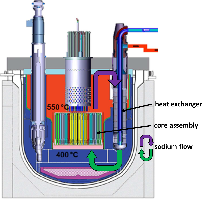
\includegraphics[width=10cm]{astrid_whole.pdf}}
    \slantedcaption{Sodium flow in the core of the current ASTRID conceptual design (taken from \cite{Barbier2017Mainoperationprocedures}).}
    \label{fig:astrid_whole}
\end{figure}

\section{State of the art of sodium flow modeling for SFR} \label{sec:stat_sod}

    In the sections above, application methods of ultrasonic monitoring for SFRs and ultrasonic properties have been briefly recalled.
Because of the dependency of sound speed on the medium temperature, as described,
it is crucial to understand the state of sodium circulation in order to estimate the usefulness and potential practical use of ultrasound measurements,
and in particular characterize the typical error levels that they can lead to for telemetry-based measurements in sodium flows.
In this section (\autoref{sec:stat_sod}), let us briefly review some of the latest studies on sodium flows in SFRs.
Pure thermo-fluid dynamical studies are cited because a thermo-fluidal
state is formed based on the history that the fluid has experienced. Our study concerns only the flow state of the upper-core region, i.e. the region located just above the
sodium outlet of the sub-assemblies. Three thermo-fluid studies will be recalled briefly in order to have knowledge on how sodium flows in the region of the core.

    \begin{figure}[htbp]
        \centerline{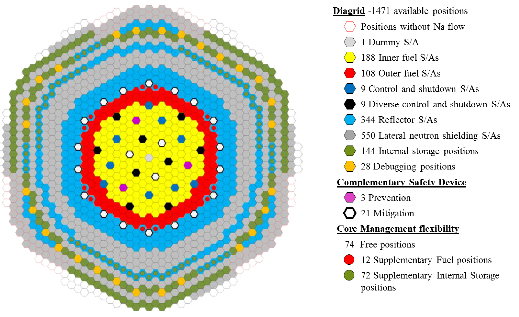
\includegraphics[width=15cm]{diagram_core.pdf}}
        \slantedcaption{Diagram for the planned ASTRID core assembly at the end of the conceptual design phase (taken from \cite{Venard2017TheASTRIDcore}).}
        \label{fig:diagram_core}
    \end{figure}
%
    In a SFR, the central part of the core is composed of hexagonal sub-assemblies that contain the nuclear fuel.
Figure \ref{fig:astrid_whole} shows the typical sodium flow in the primary coolant system,
and Figure \ref{fig:diagram_core} shows the diagram of the ASTRID core assembly at the end of the conceptual design phase.
The diameter of the core, including the reflectors, is about 7 meters, and the diameter of the vessel is about 16 meters.
The version of core design taken into account is
number four, and this version of the ASTRID core is called CFV version 4. The core assembly of version 4 is composed of 288 fuel sub-assemblies with a 17.17~cm pitch.
Each fuel subassembly includes 217 fuel pins. The diameter of the pins is 9.7~mm \parencite{Venard2017TheASTRIDcore}.
    Each pin is surrounded by helical wire spacers (Figure \ref{fig:subassembly}, B). In the core, the sodium flow orbits through the heat exchanger and core
assemblies driven by electromagnetic pumps. Inside the heat exchangers, thermal energy is passed to the secondary coolant system and then the temperature of sodium
decreases. This cooled sodium flow is heated again while the sodium flow passes through the sub-assemblies, which may have the highest temperature within
the entire cooling circuit, and which is exhausted from the subassembly heads.

    \begin{figure}[htbp]
        \centerline{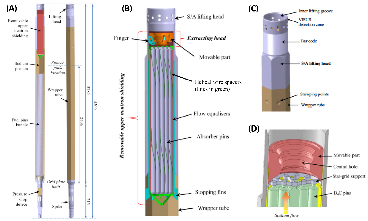
\includegraphics[width=17cm]{subassembly2.pdf}}
        \slantedcaption{Design of a subassembly. A: entire image and its cross-section. B: Neutron-shielding part. C: Subassembly head. D: Extracting head of
neutron shielding (taken from \cite{Beck2017Conceptualdesignof}).}
        \label{fig:subassembly}
    \end{figure}

    Because of the complexity of the geometry in which the sodium flow comes out, estimation for flow and heat transfer state is quite important for the
optimization of the SFR core, the subassembly design, and also for considering thermal fatigue. CEA has thus performed several numerical studies of core thermal
hydraulics of SFR by splitting them into three scales \citep{Gerschenfeld2017DevelopmentandValidation}:
    \begin{itemize}
        \item the global reactor scale, i.e. the reactor system scale,
        \item the local core scale, i.e. the individual subassembly scale,
        \item the scale of the other regions in which three-dimensional convection phenomena happen, excluding the subassembly part,
for instance the inter-wrapper gaps and the hot pool plenum.
    \end{itemize}
    This separation is currently unavoidable (in terms of computational cost) in order to be able to obtain the necessary resolution for the computation grids for each target and to maximize the volumes of the modeled domains.
    However, the interaction between the simulation of each of these scales needs to be considered because local scale phenomena may sometimes have a strong feedback effect
on the global behavior of the reactor \parencite{Gerschenfeld2017DevelopmentandValidation}.
In order to take into account all of phenomena with different scales and the interactions between them, CEA takes a calculation strategy that consists in
first computing the system-scale thermal-hydraulic states, based on a numerical code called CATHARE.
In a second step, the state of the local core scale is calculated
by taking into account the first system-scale simulation result as the initial condition.
For that step, the TrioMC code is used for the subassembly simulation, and another code called TrioCFD is used to compute the other regions in the reactor
in which three-dimensional convection occurs. Finally, once again the global-scale simulation is carried out with the data of local scale simulations
using a coupling code called MATHYS (Multi-scale ASTRID Thermal-HYdraulics Simulation).

    For example, \textcite{Saxena2014Thermalhydraulicnumerical} performed a numerical study for a subassembly of ASTRID (Figure \ref{fig:sim_subassembly})
to estimate the amount of pressure drop and hot spots (i.e. the place where temperature becomes high locally) happening around the supporting wires of fuel
pins. The pressure drop and hot spots may cause boiling of liquid sodium, and this may lead to local clad meltdown. In order to investigate the possibility of
occurrence of relatively small hot spots, \textcite{Saxena2014Thermalhydraulicnumerical} used a Large Eddy Simulation (LES) turbulent model in addition to a
Reynolds Averaged Navier-Stokes method (RANS) turbulent model.

    \begin{figure}[htbp]
        \centerline{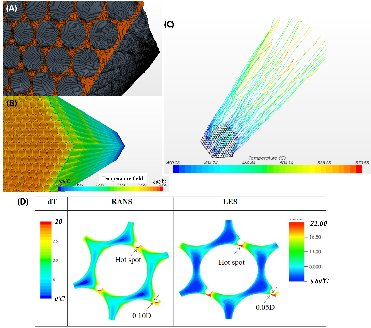
\includegraphics[width=12cm]{sim_subassembly_v2.pdf}}
        \slantedcaption{Thermal-hydraulic simulation for a subassembly made by \textcite{Saxena2014Thermalhydraulicnumerical}. A: Simulation mesh for a bundle of
fuel pins and spacing wires. B: Three-dimensional temperature field. C: Streamlines of flow with evolution of temperature (around the hexagonal can).
D: Calculated temperature difference in a cross section around a central fuel pin. The color map shows the difference of temperature based on the lowest
temperature of each cross section.}
        \label{fig:sim_subassembly}
    \end{figure}
%
    CEA is currently developing another code for the simulation of an individual subassembly model: the so-called TrioMC numerical simulation tool
(MC stands for the abbreviation of Core Model in French). This code allows one to calculate the temperature distribution of all cladding and sodium parts from a given mass flow rate.
    Figure \ref{fig:whole_core_by_trioMC}, taken from \cite{Conti2015Numericalanalysisof}, shows an example of calculation for sodium temperature of
sub-channels, i.e. spaces surrounding fuel pins, in a subassembly. The vertical axis indicates temperature values, and each color means the altitude in the
subassembly. This calculation estimates that a temperature gradient with a higher temperature at the center of the subassembly will be generated, and the radial
magnitude of the gradient will be maximum at the highest altitude, with $\Delta T$ about \num{60}\textdegree{}$C$ when $x= $\SI{0.08}{\meter}
(a more detailed figure can be found in \cite{Conti2015Numericalanalysisof}).

    \begin{figure}[htbp]
        \centerline{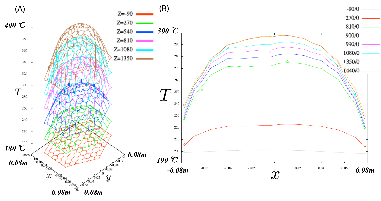
\includegraphics[width=14cm]{whole_core_by_trioMC_v4.pdf}}
        \slantedcaption{Temperature map calculated by the CEA numerical simulation code TrioMC.
A: Calculated (lines) and experimental (arrows) temperatures at each altitude of a subassembly.
B: Comparison on 2D intersections at several altitudes. The lines represent calculated values and the symbols represent experiment values. The $Z$ value is altitude in millimeters.
Taken from \cite{Conti2015Numericalanalysisof}.}
        \label{fig:whole_core_by_trioMC}
    \end{figure}
%
    After achieving the whole core temperature simulation, thermal-hydraulic calculations for the inter-wrapper and for the hot pool plenum zone are carried out by
coupling the results of the calculation of the sub-assemblies with a three-dimensional TrioCFD model (Figure \ref{fig:wholeCFD}). The thermo-fluid data for the
upper core region may then be numerically obtained, for the regions where ultrasound transducers will be installed (i.e., typically
the region shown with the purple rectangle in Figure \ref{fig:wholeCFD}).
This result illustrates the great technical and numerical challenge that needs to be addressed
to obtain quantitative information for ultrasound measurements in the upper core region,
as the above-core structure greatly modifies the sodium flow. As a result, the state of the flow and the distribution of the thermal gradient become heterogeneous.
From the temperature dependency, which has been recalled in \autoref{ssec:ac_prop}, these complex heterogeneities lead to uncertainty/difficulty of ultrasound measurements
in the upper-core region. This thesis will thus focus on how to try to compute and analyze such complexity and uncertainty.

    \begin{figure}[htbp]
        \centerline{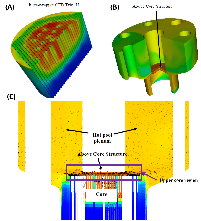
\includegraphics[width=17cm]{wholeCFD.pdf}}
        \slantedcaption{A,B: 3D TrioCFD model of inter-wrapper model and the hot pool plenum, including the upper-core region. C: Calculated temperature map
(color scale) and flow state (arrows). Taken from \cite{Conti2015Numericalanalysisof}.}
        \label{fig:wholeCFD}
    \end{figure}
%
    A more detailed numerical study on the flow state at a subassembly head was carried out by \textcite{Beck2017Conceptualdesignof}. The aim of that study was
design optimization of pins configuration and geometry of the extraction head (Figure \ref{fig:subassembly}). In Figure \ref{fig:cfd_head}, pre-optimization and
optimized geometry and simulated flow and temperature fields are shown. From the results for the pre-optimization geometry, the maximum difference of temperature at the
position of the monitoring system (A.2-2) is about \num{20}\textdegree{}$C$.
From the results for the optimized geometry, the size of the temperature gradient (B.2-2) at the same position is about \num{7}\textdegree{}$C$
and the velocity magnitude field (B.1-2) is more homogeneous than the pre-optimization result (A.2-1).
    We consider that, in reality, the state of the sodium flow becomes more complex than these calculation results
because of the effect of mixing with colder sodium around the outlet of a subassembly, and also because of convection.
Let us also mention that a Reynolds Averaged Navier-Stokes (RANS) model is used as the turbulent model, which means that the resulting size of the
heterogeneities is averaged for the point of view of ultrasounds, i.e. the size of the wavelength being much smaller than the resulting size of heterogeneities in the CFD results
for a sodium flow in the SFRs that are currently available.

    \begin{figure}[htbp]
        \centerline{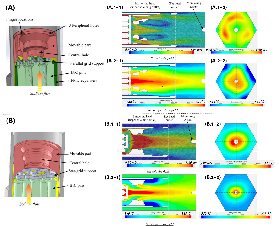
\includegraphics[width=17.9cm]{cfd_head_v3.pdf}}
        \slantedcaption{Geometry A: before optimization of an inner head of a subassembly; cross-sectional flow field (A.1-1) and temperature field (A.2-1) in the
long axial direction, and velocity magnitude field (A.1-2) and temperature field (A.2-2) in a perpendicular cross-section at the position of the monitoring system,
i.e. at the place where the thermocouples and flow-meter are located. B: after optimization: cross-sectional flow field (B.1-1) and temperature field (B.2-1) in the long axial direction,
and velocity magnitude field (B.1-2) and temperature field (B.2-2) in a perpendicular cross-section, taken from \textcite{Beck2017Conceptualdesignof}.
The inner diameter of the head is \SI{15}{\centi\meter} and the length of the cylindrical part (not hexagonal) of the head (i.e. from the left boundary of the A.1-1 image to the "S/A head outlet" part) is \SI{27}{\centi\meter}.}
        \label{fig:cfd_head}
    \end{figure}

    The latest numerical analysis, which was carried out by CEA for the upper core region and the hot pool plenum at nominal reactor power, shows that the possible radial flow rate is
about \SI{4.5}{\meter\per\second}, and the maximum variation rate of radial temperature is about \num{23.4}\textdegree{}C par \SI{10}{\centi\meter}
\parencite{Haubensack2016Calculsthermohydrauliquesdu}. It also shows that the modification of the acoustic field depends on the three-dimensional angle
and curvature of the temperature gradient versus a direction of an acoustic propagation ray.
    For this reason it is necessary to take into account the medium heterogeneities to ensure the accuracy of acoustic measurement methods
\parencite{Massacret2014Etudedunemethode}.
%
    The main objective of this thesis is thus going to be to study how an acoustic wave propagates in a model of a sodium flow that has realistic heterogeneity.

\section{Thermal-hydraulics studies with fluctuation of sodium jets, and acoustic point of view}

    As mentioned above, several thermal-hydraulic studies on the state of the sodium coolant fluid in the primary circuit of SFR have been carried out in the
literature. These studies, except \textcite{Saxena2014Thermalhydraulicnumerical}, use the Reynolds-Averaged Navier-Stokes (RANS) model for their
turbulence model for the upper core domain, which is the place on which we want to focus in this thesis.
    Turbulence models generally used for computational fluid dynamics (CFD) may be broadly divided into three types: RANS, Large-Eddy Simulation (LES),
and Direct Numerical Simulation (DNS). The appropriate model to use in a given situation is selected based on the purpose of the simulation (for instance the level of accuracy needed etc.)
and the amount of computer resources required:
%
\vspace{-4mm}
    \begin{itemize}
    \item RANS divides the flow variables (i.e. velocity, pressure and temperature) into a time-averaged part and a fluctuating part (a process called
Reynolds decomposition), and then a time-averaged thermo-fluid field is calculated,
    \item LES defines a cut-off threshold on the spatial size. Eddies larger than this threshold are calculated directly, and the smaller eddies are
modeled and calculated as more isotropic ones than those directly calculated,
    \item DNS solves the set of equations without any approximation, thus this model has the highest resolution and accuracy among these three models. However this method
requires enormous amounts of computer resources and this is why the application of DNS for the analysis of a whole nuclear core or a large part of a nuclear
core is currently still not feasible (but will become feasible one day).
    \end{itemize}

\vspace{-4mm}
    Figure \ref{fig:turbulent_models} shows the schematic representation of turbulent models and numerical results of each model
(\cite{Poitou2009Modelisationdurayonnement}, \cite{Saxena2014Thermalhydraulicnumerical}).
From this figure it is clear that a RANS-based simulation would not give a description of the temporal fluctuations of the jets.
    The acoustic wavelength of \SI{1}{\mega\hertz}, which is one of the possible acoustic frequencies considered to be used in the ASTRID core, is small:
approximately \SI{1}{\milli\meter} in the operating situation. This is the reason why a thermal-hydraulic field that would be averaged too much
may sometimes not be suitable to perform realistic acoustic simulations, because the spatial and temporal resolutions of averaged thermal-hydraulic results
are coarser than the resolution of the acoustic simulations.

    As we recalled in the previous sections, in the upper core region, hot sodium jets, which have a temperature within the range \num{450}\textdegree{}C (control rod) to \num{550}\textdegree{}C (hotter subassembly), and ambient
sodium, which may be \num{50}\textdegree{}C colder than the hottest jets, are mixed. This can cause complex and poorly known thermal-hydraulic phenomena.
For this reason, several studies exist on the thermo-fluidal fluctuation of sodium jets. The main purpose of these studies is the observation of a mixing phenomenon in the jets
of liquid sodium, and estimation of thermal fatigue of the metal material that is present in a SFR core. In those studies, the thermal fluctuation cycle is investigated in
details, thus we may use these results for our acoustic studies, as there are similarities with the objectives of our study.

    \begin{figure}[htbp]
        \centerline{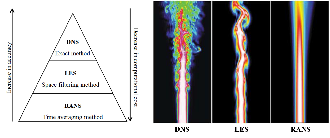
\includegraphics[width=12cm]{turbulent_models.pdf}}
        \slantedcaption{Left: Schematic representation of the three classical types of turbulent models used in numerical simulations.
Right: modeling of a flame. Taken from \cite{Poitou2009Modelisationdurayonnement} and \cite{Saxena2014Thermalhydraulicnumerical}.}
        \label{fig:turbulent_models}
    \end{figure}

\vspace*{-7mm}
    \begin{figure}[htbp]
        \centerline{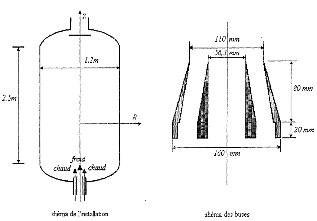
\includegraphics[width=12cm]{najeco_v2.pdf}}
        \slantedcaption{Test section of the NAJECO loop (taken from \cite{Tenchine1994Jetscoaxiaux:}).}
        \label{fig:najeco}
    \end{figure}

\vspace*{-3mm}
\subsection{The NAJECO experiment}

    In order to determine the characteristic length $L_{\theta}$ of these thermal heterogeneities in different fluids, \cite{Tenchine1994Jetscoaxiaux:} and
\cite{Tenchine1994Jetscoaxiaux:a} performed several experiments in the NAJECO and AIRJECO test loops. The objective of these experiments was to determine the
similarities between the thermal fluctuations of a flow of sodium and a flow of air and to determine if air is appropriate for the simulation of sodium with
temperature heterogeneity. To this end, the two test sections had identical geometries and generated coaxial fluids at different temperatures.

    For the NAJECO experiment, the two concentric sodium jets have different temperatures and flow rates: \SI{150}{\cubic\meter\per\hour} at
\num{280}\textdegree{}C and \SI{30}{\cubic\meter\per\hour} at \num{200}\textdegree{}C. The trial section of this loop is represented in Figure \ref{fig:najeco}.
    This test section generates two coaxial jets at different temperatures, and thus generates thermal heterogeneities that can be encountered at the
subassembly outlet, mainly where the coaxial jets from sub-assemblies and inter-sub-assemblies mix. The study of this experiment makes it possible to better
understand which types of heterogeneities may develop above the reactor core.

    In this experiment, a thermocouple was placed with the aid of a pole at different points of the flow, which made it possible to record temperature
fluctuations, to measure the spectrum of the thermal fluctuations, and to deduce the characteristic lengths of the flow.
    Table \ref{table:najeco} shows the results of this experiment at a distance of \SI{0.05}{\meter} from the sodium outlet.
    $U$ is the speed of the flow at the measurement point and $R$ is the distance from the measurement point to the vertical axis (Figure \ref{fig:najeco}).
    The characteristic length of the temperature fluctuation $L_{\theta}$ is calculated from the measured values based on
    \begin{align}\label{eq:I_4}
        L_{\theta} = \frac{U}{2\pi f_{\theta}},
    \end{align}
    where $f_{\theta}$ is the peak frequency of the measured temperature temporal fluctuation.

    \begin{table}
        \centering
        \slantedcaption{Characteristic length of the thermal heterogeneities at different points of the flow, 50~cm above the nozzles
(taken from \cite{Tenchine1994Jetscoaxiaux:}).}
\vspace{5truemm}
        \begin{tabular}{lll}
        Radius $R$ [\si{\meter}] & Speed $U$ [\si{\meter\per\second}] & Length $L_{\theta}$ [\si{\meter}] \\ \hline
        \num{0}              & \num{1.05}                 & \num{0.037}                    \\
        \num{0.016}          & \num{1}                    & \num{0.039}                    \\
        \num{0.04}           & \num{0.8}                  & \num{0.032}                    \\
        \num{0.10}           & \num{0.3}                  & \num{0.024}                    \\
        \end{tabular}
        \label{table:najeco}
    \end{table}

    Thus, for a sodium flow of this type, the characteristic length of the thermal heterogeneities \SI{50}{\centi\meter} above the tubes discharging the sodium
ranges between \SI{2}{\centi\meter} and \SI{4}{\centi\meter}. It is also important to note that heterogeneity size decreases with increasing distance between
the measurement point and the center of the flow. To understand why these variations occur, radial and axial measurement of the temperature fluctuations were
performed in the NAJECO experiments; the results are presented in Figure \ref{fig:najeco_res}.
    This profile indicates that most of the thermal fluctuations do not occur in the axis of the exit flow but rather on a ring centered on the flow, where the two
coaxial jets mix. On both sides of this ring the temperature heterogeneities are thus smaller. It should be noted that these profiles are also given far from
the jet outlets (\SI{50}{\centi\meter}).

    These results show that in spite of the high thermal conductivity of sodium, which tends to homogenize the medium temperature,
thermal heterogeneities can be observed as a result of the flow velocity field. These experimental results would not be simply compared to the expected SFR
sodium flow, as the direction of the flows are not identical.
Nevertheless it is likely that, in a horizontal plane very close to the subassembly outlet, circular homogeneous temperature zones can be observed,
their radius being of the order of that of the assembly. These zones would be separated by zones in which the temperature fluctuations
are large and the characteristic size of the temperature heterogeneities is about a few centimeters.

    It should also be noticed that these experiments were run without any obstacle and high above the jet outlets, the flows implemented here being different
from those implemented in the case of a actual reactor in which sodium flows are disturbed by the upper-core structures situated about 40~cm above the assembly
outlet. The findings of this study may therefore be modified by the presence of the upper-core structures. More precise knowledge of the flow above the core
will be necessary to conclude on the presence of a small disturbed zone above the assemblies.

    \begin{figure}[htbp]
        \centerline{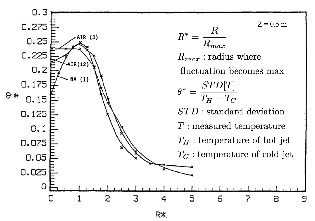
\includegraphics[width=13cm]{najeco_res_v4.pdf}}
        \slantedcaption{Radial profile of the intensity of the fluctuations in sodium, indicated as NA(1), and in air, indicated as AIR(3) and AIR(12), at altitude $Z$ = \SI{0.5}{\meter}
(taken from \cite{Tenchine1994Jetscoaxiaux:}).}
        \label{fig:najeco_res}
    \end{figure}

    \begin{figure}[htbp]
        \centerline{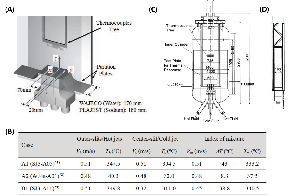
\includegraphics[width=16.2cm]{plajest_jaea_v2.pdf}}
        \slantedcaption{Geometry of the PLAJEST experiment (A,C,D) and three different initial conditions of the flow state (B), taken from \cite{Kobayashi2015Proposalofbenchmark}.
Water (A2) and sodium (A1, B1) are used for each medium.}
        \label{fig:plajest_jaea}
    \end{figure}

\subsection{The PLAJEST experiment, and numerical modeling based on large-eddy simulation}
\label{ssec:PLAJEST}

    Another program, called PLAJEST, is a collaboration between the Japanese Atomic Energy Agency (JAEA), the U.S. Department of Energy (DOE), and CEA in France.
The main purpose of PLAJEST is to observe heat conduction at a liquid-solid boundary in a sodium cooling circuit, because the thermal fluctuations lead to
high-frequency thermal fatigue and thus possibly to cracks in adjoining structures of SFRs. The configuration of this experiment is shown in Figure
\ref{fig:plajest_jaea}. After the experiment made by JAEA \citep{Kimura2005Studyonconvective,Kimura2008Studyonthermal}, thermo-fluid analysis was
done by CEA in its Service de thermo-hydraulique et de m\'ecanique des fluides (STMF) (\cite{Angeli2015LargeEddySimulation}, Figure \ref{fig:plajest_cea}). In that analysis, the results A and B indicate a good fit on time-averaged
normalized temperature (A) and its fluctuation (B) between experimental and numerical values. Moreover the power spectral density curves of temperature at the
middle point of the domain under study also exhibit a good fit (D).

    While these PLAJEST studies are not based on ultrasound propagation, and we did not carry out an acoustic experiment with the PLAJEST configuration
in this thesis, we will use the thermo-fluid computation results of case A1 as a CFD simulation results that is well validated by the experiment for our
full-wave propagation numerical simulations (in Chapter \ref{chap:3}) in realistic conditions.
CEA/STMF used a Large-Eddy Simulation turbulence model for this simulation, thus we may utilize these temperature fields with higher spatio-temporal resolution.

\subsection{Thermal fluctuation models used in previous acoustic studies in the literature} \label{ssec:fluc_mod}

    In previous studies published in the literature on acoustic wave propagation in heterogeneous liquid sodium,
a stochastic modeling was always applied for modeling of medium fluctuations
and heterogeneities of sodium flow in SFRs, because pertinent thermal-hydraulic input data were not available, and/or because realistic numerical modeling was too complex
or too expensive to perform. This stochastic method is still the fastest and cheapest way to prepare a
fluctuating acoustic propagation medium. Several such studies are briefly recalled in this section.

    David Fiorina, in his PhD thesis \parencite{Fiorina1998Applicationofthe}, generated fluctuating fields of sound velocity based on isotropic and homogeneous
Gaussian random processes in 2D.
This technique allows for a high-resolution representation of random variations in the propagation medium (\parencite{VladimirE.Ostashev2015AcousticsMovingInhomogeneous}).
He studied the effects of this heterogeneity in the propagating medium on an acoustic wave using a Gaussian beam summation
method. A point and line source were used in his calculation, and he analyzed the effect on the acoustic rays, time-of-flights, and variance of sound intensity
(Figure \ref{fig:fiorina}). In that simulation, the medium used was water. The average temperature was \num{30}\textdegree{}C, and variance of the temperature
was \num{25}\textdegree{}C with $L_{\theta}=0.03\, \text{m}$. He concluded that when the propagation distance is shorter than about \num{34} times the value of
$L_{\theta}$ (the characteristic length of heterogeneities), the simulated curve and the theoretical solution are in very good agreement. However, when the propagation distance
becomes longer than that length, the difference between the analytical solution and the result of the calculation becomes larger.
Let us mention that in this thesis, a Gaussian random process following this approach will be used in Chapter~3.

    Then, \textcite{Iooss2000Statisticalmomentsof} extended this method to a geometrically-anisotropic homogeneous Gaussian random process in 2D. This
extension was motivated by the demand coming from the fact that the fluctuation pattern is not isotropic when the flow velocity is not small. The Gaussian beam
summation method was again applied in that study, and the case of a plane wave and then a spherical wave were examined as types of acoustic emission.
Figure \ref{fig:iooss} shows the isotropic temperature and flow velocity fields (A) and anisotropic sound celerity field (B).
In \textcite{Iooss2002Numericalsimulationof} the authors concluded that:
    \begin{itemize}
        \item  In 3D modeling, the effects of the mean and turbulent fields are theoretically stronger on the travel times than in 2D modeling,
        \item  A fluctuating pattern generated based on a stochastic model is far from realistic fluctuating patterns,
        \item  Deterministic fluid mechanics can provide realistic temperature and velocity fields.
    \end{itemize}

    \begin{figure}[htbp]
        \centerline{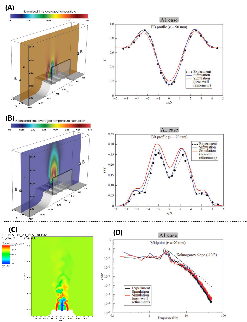
\includegraphics[width=17cm]{plajest_cea_v2.pdf}}
        \slantedcaption{Computational Fluid Dynamics results for the A1 case of the PLAJEST experiment configuration, obtained by \cite{Angeli2015LargeEddySimulation}.
A: Time-averaged normalized temperature field and
comparison with experimental data. B: Time-averaged normalized temperature fluctuation and comparison with experimental data.
C: Example of a non-time-averaged temperature field at a given time. D: Power spectral density curve at the middle point of the studied domain.}
        \label{fig:plajest_cea}
    \end{figure}

    \begin{figure}[htbp]
        \centerline{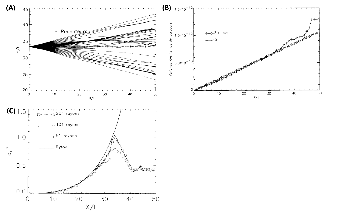
\includegraphics[width=17cm]{fiorina.pdf}}
        \slantedcaption{Results of a Gaussian summation simulation obtained by \textcite{Fiorina1998Applicationofthe}. A: Calculated acoustic rays emitted from
a point source. The value of each axis is divided by the characteristic length of fluctuations $L=L_{\theta}$. B: Variance of time-of-flights versus
propagation length. C: Normalized variance of fluctuations of sound intensity ($\sigma_T(\bm{x})^2=\sum_i(I_i-I_{average})/I_{average})^2, I_i=p_i*|\bm{v_i}|,
i: \text{index for } $x$ \text{ positions}, p: \text{pressure}, \bm{v}: \text{velocity vector}$) versus propagation length, compared with Rytov approximation \cite{Beydoun1988FirstBornRytov}. Taken from
\textcite{Fiorina1998Applicationofthe}.}
        \label{fig:fiorina}
    \end{figure}

    \begin{figure}[htbp]
        \centerline{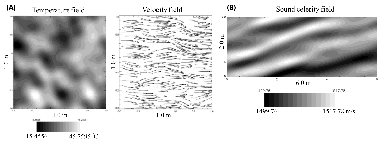
\includegraphics[width=17cm]{iooss_v4.pdf}}
        \slantedcaption{A: An example of isotropic temperature and flow velocity fields of water. B: Anisotropic sound celerity field in liquid sodium.
The velocity of the ambient flow is \SI{16}{\meter\per\second} tilted at \num{11.5}\textdegree{}. Taken from \textcite{Iooss2000Statisticalmomentsof}.}
        \label{fig:iooss}
    \end{figure}

    \cite{Lue2011Modelisationdela} and \textcite{Lue2012Stochasticsimulationof} applied a Gaussian random process to 3D simulation, and also proposed to apply
the Gaussian random process not to the generation of a physical quantity field (i.e. temperature and flow velocity field) but rather to the propagation field
(i.e. times of flight and acoustic amplitudes) itself. In these works, the propagation field is first calculated as wave propagation in a homogeneous medium,
and then the heterogeneous effects are calculated in transversal planes (Figure \ref{fig:bo} A) as a function of propagation distances, and then added to
the homogeneous fields.
Figure \ref{fig:bo}B shows an example of time-of-flight fluctuations in the transversal plane at a distance from the source of $30 l_\epsilon$,
where $l_\epsilon$ is the characteristic length of the medium fluctuations.
Sub-figure~C is an example of a fluctuating acoustic field calculated based on the stochastic model that we use.
A circular transducer with diameter \SI{30}{\milli\meter} was used.
The source signal is a Gaussian-modulated sinusoidal pulse with a dominant frequency of \SI{2}{\mega\hertz}.
D: Profiles of amplitude at $x$ = \SI{1.4}{\meter} extracted from the results presented in~C.
The red curve shows the result obtained in the case of homogeneous medium conditions.

\textcite{Lue2012Stochasticsimulationof} called this method a stochastic method.
The stochastic method provides faster generation of the fluctuating propagation field than a deterministic method.
The size of the calculated volume in that work is \SI{0.1}{\meter} < x < \SI{1.4}{\meter} and \SI{-0.05}{\meter} < y < \SI{0.05}{\meter}, with 2000 calculation points.
For the deterministic model the calculation time was about \SI{1.5}{\hour}, while for the stochastic model it was only \SI{10}{\second}, i.e., more than 500 times cheaper.
The results taken from that paper and presented in Figure~\ref{fig:bo}~D show a mean deviation of about \SI{10}{\milli\meter}
and a standard deviation of about \SI{7.6}{\milli\meter} at $x$ = \SI{1.4}{\meter}.
Let us mention that the stochastic method in \textcite{Lue2012Stochasticsimulationof} was validated using a ray-tracing technique.

    \begin{figure}[htbp]
        \centerline{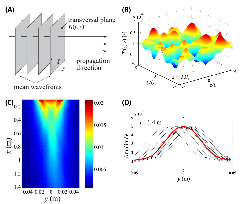
\includegraphics[width=17cm]{bo_v2.pdf}}
        \slantedcaption{
            A: Definition of the transversal plane on which the fluctuating part of a propagation field is calculated.
            B: Time of flight fluctuation on a transversal plane.
            C: One of fluctuating acoustic field calculated based on the stochastic model.
            D: Profiles of Amplitude at x = \SI{1.4}{\meter} extracted from C.
            Taken from \textcite{Lue2012Stochasticsimulationof}.}
        \label{fig:bo}
    \end{figure}
%
    \textcite{Massacret2014Etudedunemethode} simulated wave propagation just above the heads of the sub-assemblies under the assumption that in this region the
fluctuation of the medium is weak enough and can thus be ignored.
    The only heterogeneity taken int account is a static heterogeneous temperature that creates a temperature gradient along the wave path.
    His results show that under such an assumption, acoustic rays may be affected significantly and deviated (Figure \ref{fig:nicolas}). A ray-tracing code
called AcRaLiS was developed for this simulation. To describe the temperature field, the author performed an interpolation of the physical values of the field
onto the spatial points that are used for the ray-tracing calculation using a Delaunay triangulation.
    \textcite{Massacret2014Etudedunemethode} also applied the temperature and flow velocity map calculated for the PLAJEST experiment based on a RANS turbulent model (see the above section)
and obtained estimates of the change of times of flight for the wave front.
    \begin{figure}[htbp]
        \centerline{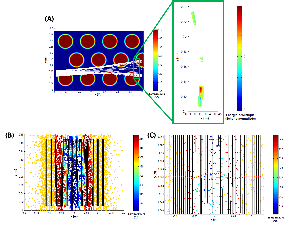
\includegraphics[width=17.9cm]{nicolas_v2.pdf}}
        \slantedcaption{A: Acoustic rays obtained based on a ray-tracing simulation code called AcRaLis above the subassembly heads without fluctuations (left)
and acoustic energy 63~cm away from the acoustic source (right). B: Deviated acoustic rays calculated with a temperature field obtained from the PLAJEST
simulation data. C: Plotted wave front. Taken from \textcite{Massacret2014Etudedunemethode}.}
        \label{fig:nicolas}
    \end{figure}

    To finish the overview of previous studies, let us mention some studies currently being performed in Belgium.
    SCK-CEN, the Belgian Nuclear Research Center is currently developing MYRRHA, a Generation-IV liquid-metal-cooled research nuclear reactor
\parencite{AitAbderrahim2012MYRRHAAmulti}. Lead-bismuth eutectic, which is also optically opaque, is used as the coolant medium in this reactor.
    In this project, one of the possible applications of the acoustic measurement technique is the detection and localization of potentially lost fuel assemblies.
For this purpose, the acoustic propagation distance may be about \SI{2.5}{\meter} and thus the effects of the heterogeneous temperature and velocity fields
on acoustic wave propagation need to be examined.
    To do this, \textcite{VandeWyer2014Experimentalandnumerical} developed an experimental facility called TAUPE. Water is used as the propagation
medium in that experiment (Figure \ref{fig:taupe} A,B). The corresponding medium, in terms of flow velocity and temperature gradient, were simulated in TAUPE,
and acoustic wave propagation was observed by means of acoustic signal and shadow-graph visualization.
    The authors of this experiment also developed a ray-tracing code and validated it based on their experimental results.
    They concluded that their ray-tracing code estimates the effects of temperature gradients on wave propagation accurately (Figure \ref{fig:taupe} D),
while the effects of the flow velocity field are overestimated. As \cite{Massacret2012Simplifiedmodelingof}, they also concluded that the effect of the flow velocity field
is negligible but that the effect of the temperature gradient is not negligible when the propagation distance is greater than about \SI{2.5}{\meter},
which is the required length for object detection and visualization.

    \begin{figure}[htbp]
        \centerline{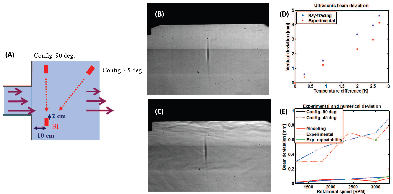
\includegraphics[width=17cm]{taupe_v2.pdf}}
        \slantedcaption{A: Configurations of the TAUPE experiment. S1 is the emitter. Two angles of acoustic propagation direction are examined.
B: Visualized wavefront in water without a temperature gradient nor velocity field. C: Visualized wavefront in water with a temperature gradient and velocity field.
D: Comparison between experimental results
and calculations made based upon a ray-tracing code, depending on the temperature gradient. E: Comparison between experimental results
and calculations made based upon that ray-tracing code, depending on the rotation of the flow generator.
Taken from \textcite{Wyer2015Theeffectof}. The authors find that the amount of (vertical) beam deviation increases when the magnitude of the temperature gradient becomes larger.
The same trend is also found when the rotational speed of the flow generator becomes faster, i.e. when the flow speed becomes faster.}
        \label{fig:taupe}
    \end{figure}

\section{Summary of the main goals of this thesis} \label{sec:goals}

    The main goals of this thesis are thus:
    \begin{itemize}
        \item The development and application of a full-wave propagation numerical method for the numerical analysis of acoustic wave propagation in the sodium coolant of a SFR,
for the first time in the literature to our knowledge. We selected the spectral-element method (SEM), which is a type of high-order time-domain finite element method.
As described above, to our knowledge only ray-based methods have been applied so far in the literature for acoustic wave propagation in such a medium,

        \item Improving the sodium flow description to take into account spatial fluctuations of the medium at the ultrasonic scale,

        \item Using the latest development of CFD calculations for sodium flows made by Service de thermo-hydraulique et de m\'ecanique des fluides (STMF) at CEA, we will study the effect of not only taking into account a 3D environment but also
temporal variations of the heterogeneities and fluctuation of liquid sodium on acoustic wave propagation. Time slices of the temperature field will be
used to describe the medium conditions for our acoustic simulations.
    \end{itemize}
     Such developments should thus help the acoustic community to improve knowledge on these aspects, for instance for the design of future ultrasonic measurement devices in such environments.

    In Chapter 2, we will recall basic properties of the modeling methods (i.e. SEM, Finite Difference Time Domain methods (FDTD) and ray methods) for acoustic
wave propagation.

    In Chapter 3, we will first perform a comparative study between SEM and FDTDs for acoustic wave propagation in a thermally-heterogeneous medium, in order
to validate our numerical simulation techniques. We will then perform a two-dimensional simulation study based on the spectral-element method
to investigate in detail the possibility of performing acoustic thermometry for sodium jets.
A Gaussian random process method will be used to represent the thermal fluctuations.

    In Chapter 4, we will introduce and develop a three-dimensional acoustic wave propagation simulations, again based on the spectral-element method but
in the significantly more difficult three-dimensional case this time, and will analyze its results.
Temperature fields calculated for the PLAJEST geometry by CEA STMF Saclay, and with a Large-Eddy Simulation turbulent model, will be used as input.
The amount of possible deviation of acoustic waves resulting from variations of the temperature field with time will be analyzed and discussed.

    In Chapter 5, we will finally draw conclusions and will discuss future studies.

